\documentclass{article}
\newcommand*{\qed}{\hfill\ensuremath{\blacksquare}}
\usepackage{amsmath}
\usepackage{amssymb}
\usepackage{graphicx}
\graphicspath{{.}}

\title{Computational Linear Algebra, Assignment 1, Part I}
\author{Maya Shende}
\date{Due: February 21st, 2018}

\begin{document}
\maketitle

\begin{enumerate}

	\item For vectors \textbf{u} and \textbf{v}, proved a geometric proof that $|u + v| \leq |u| +|v|$. \\
	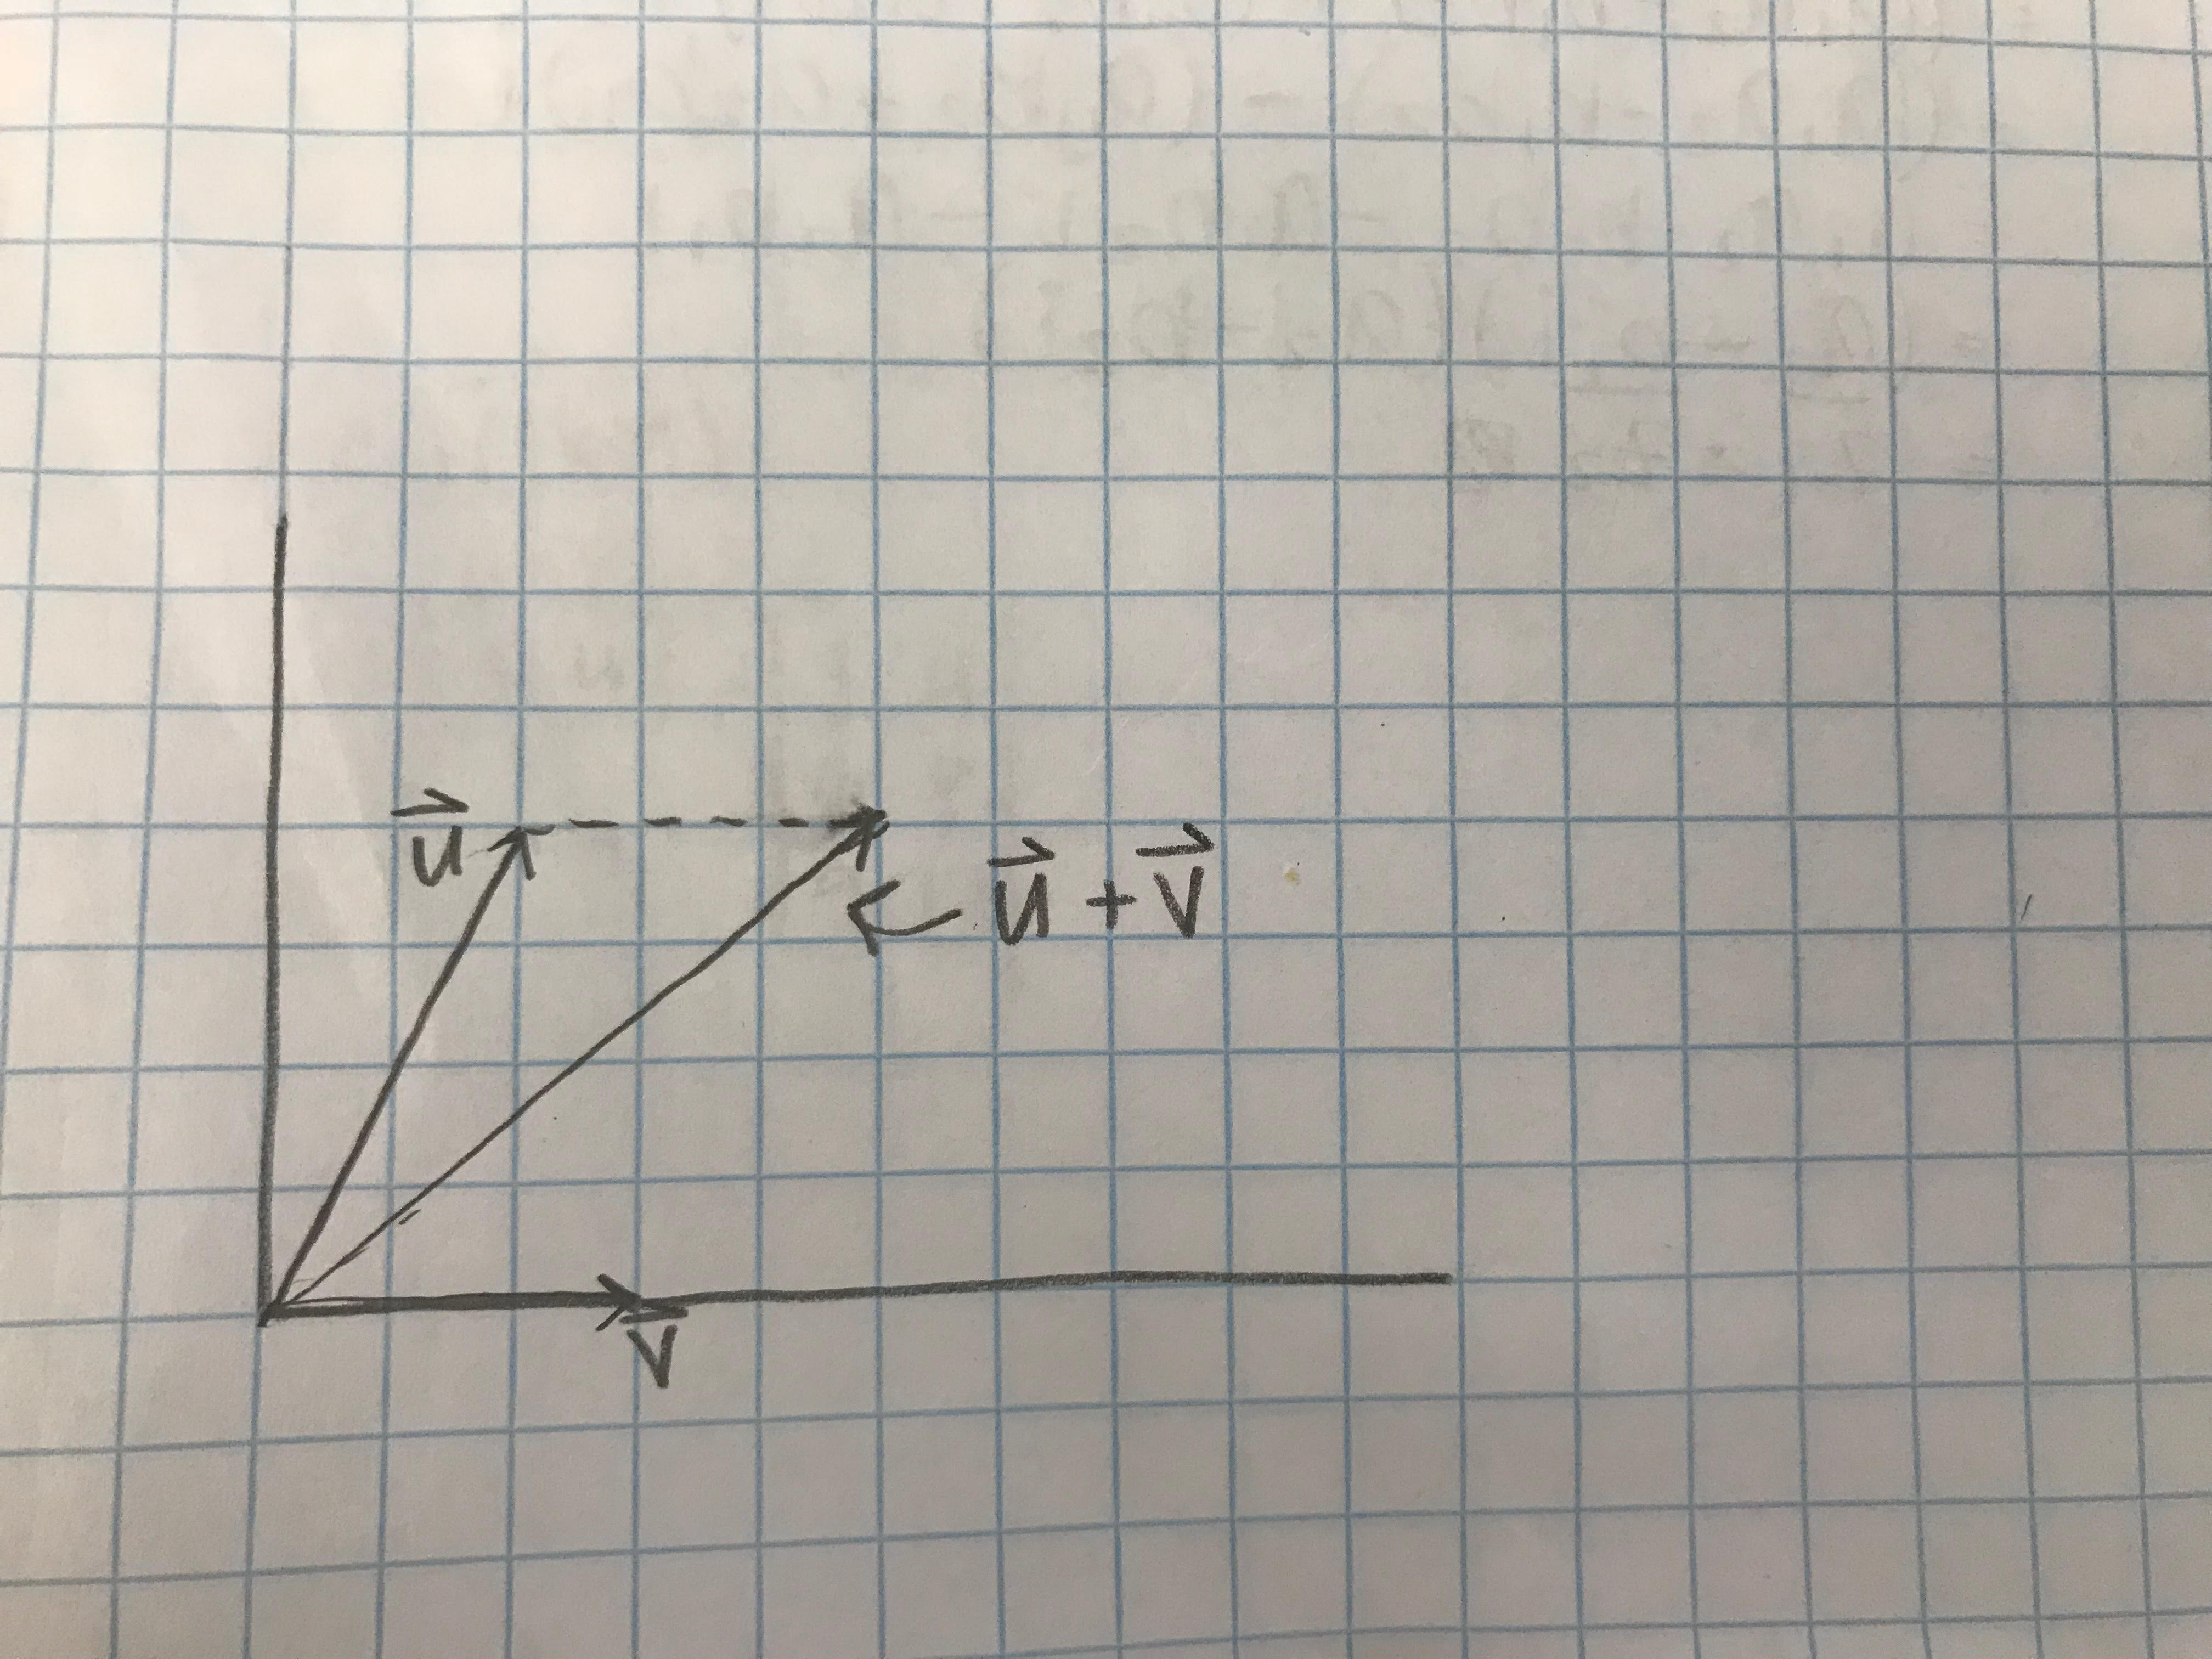
\includegraphics[scale=0.05]{problem2}\\
	If we look at this image, we see two vectors \textbf{u} and \textbf{v} plotted head to tail to form a parallelogram. In doing this, we can see that the traversal along the vectors \textbf{u} and \textbf{v}  individually will lead to a longer length than if we were to just traverse the vector representing the addition of the two original vectors. This can also be stated as the shortest path between two points is the straight line formed by the two points. 
	
	\item What is the implication for complex numbers? Can the same idea lead to the conclusion that $|z_1 + z_2| \leq |z_1| + |z_2|$? \\
	\textbf{Solution: } Assuming the shortest path is a straight line between two points, we can extend this concept to complex numbers, in which we treat the axes as the real and imaginary parts of the complex number.
	
	\item What can you conclude about the size relationship between $|u \cdot v|$ and $|u||v|$? Is one always less than the other?\\
	When $\theta = 0$, we see that $|u \cdot v| = |u||v|$. When $\theta = \pi / 4$, we see that $|u \cdot v| < |u||v|$, and when $\theta = \pi / 2$, we have that $|u \cdot v| = 0$. Based on this, we can see that there are two relationships that are both dependent on the range of the value of theta. So, we have: \\
	When $0 \leq \theta \leq \frac{\pi}{2}$ and $\frac{3\pi}{2} \leq \theta \leq 2\pi$, $|u \cdot v| \leq |u||v|$. Otherwise, $|u \cdot v| > |u||v|$. 


\end{enumerate}

\end{document}